\section{Integration and Test Plan}
As already stated before, the development and testing of D4H must be completed before starting to implement ASOS and T4R, so the development team effort should be focused on that application first. Afterwards, ASOS and T4R can be implemented and integrated in parallel. \\
Note that only the server-side is described here, but also the presentation and graphical interface in the Client should be brought on feature by feature, so as to have them fully completed one by one. \\
On the other hand, the database is the first element that should be completed, since every other component (directly or indirectly) depends from it.

The details concerning the functioning of the software components will not be further discussed here, since they have already been presented in \textbf{section \ref{ComponentView}}.

\subsection{Data4Help}
    There are five features that can be identified in D4H, as shown in the \textbf{figure \ref{fig:D4H_DependencyDiagram}}. Each of them is identified with a colour and mapped to the components needed to offer it.
    
    \begin{figure}[htbp]
        \centering
        \makebox[\textwidth][c]{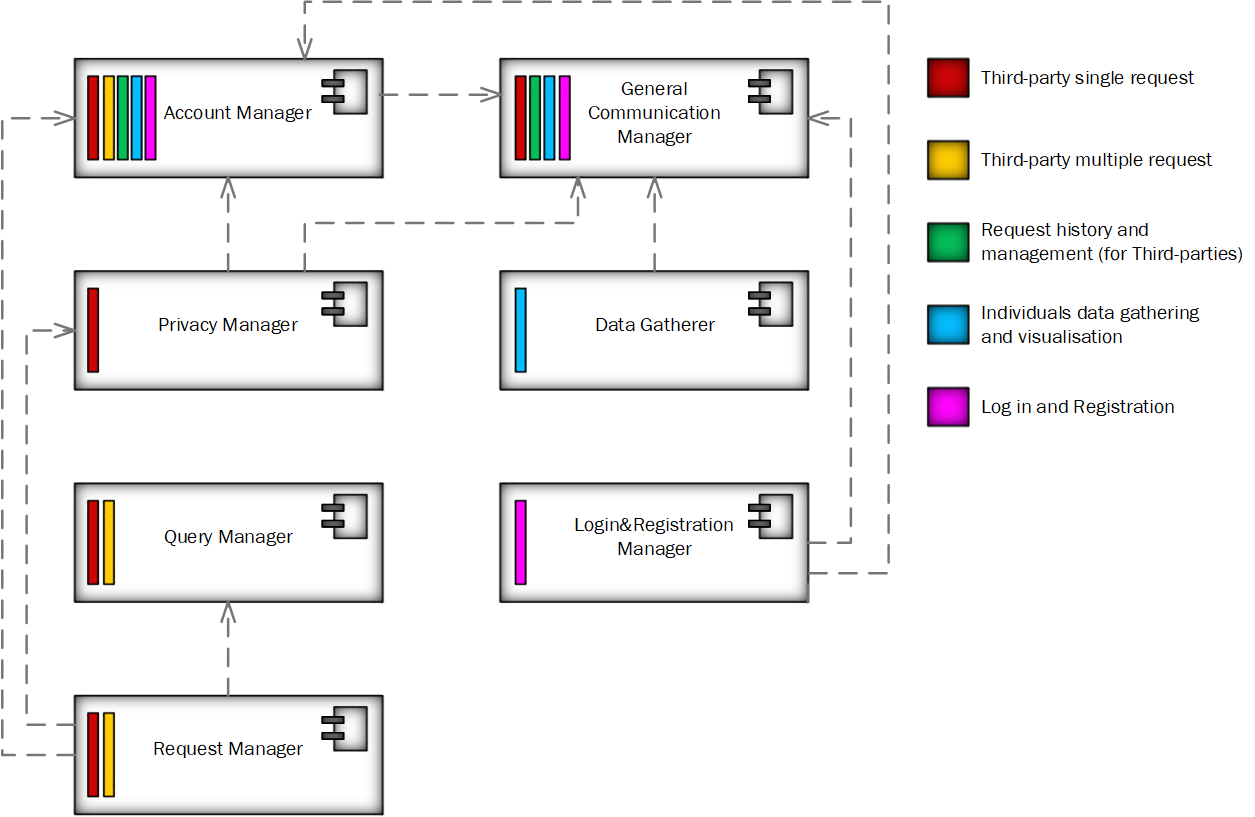
\includegraphics[scale=0.45]{pictures/D4H_DependencyDiagram.png}}
        \caption{Dependencies among D4H components}
        \label{fig:D4H_DependencyDiagram}
    \end{figure}
    
    The development will be carried on with a thread for each feature, in order of importance.
    
    \begin{enumerate}
        \item \emph{Data gathering and visualisation}
    \end{enumerate}
    The first one to focus on is the data gathering from Individuals and their visualisation (light blue rectangle in the \textbf{figure \ref{fig:D4H_DependencyDiagram}}). Completing this would allow to have real sampled data to be used for the next functionalities. In order to do so, the part of the General Communication Manager in charge of delivering the acquisition data messages must be developed, along with the Data Gatherer, as a whole, for their processing and storing. As for the visualisation of these data, even the part of the Account Manager that retrieves them from the database has to be completed. Also in this case, the General Communication Manager acts like a switch, forwarding the message.
    
    \begin{enumerate} [resume]
        \item \emph{Third-party single request}
    \end{enumerate}
    Having now the capability of acquiring Individuals' data, the second feature to focus on is the single data requests, and possible subscriptions, performed by Third-parties (red rectangle in the \textbf{figure \ref{fig:D4H_DependencyDiagram}}), because it involves several component and it is more likely to face difficulties in implementing it. The interested components are:
        \begin{itemize}
            \item Request Manager for the request processing;
            \item Query Manager for data retrieval from the database
            \item Privacy Manager to ask for the Individual's approval;
            \item Account Manager to handle subscriptions;
            \item General Communication Manager to route the messages.
        \end{itemize}
    The sections of these components that deal with this type of request have to be fully integrated and tested at this point. Note that the Privacy Manager is only used for this functionality, so it must be fully implemented and tested in this phase.
    
    \begin{enumerate} [resume]
        \item \emph{Third-party multiple request}
    \end{enumerate}
    At this point the feature that allows Third-parties to perform group searches, with eventual subscriptions, can be implemented (yellow rectangle in the \textbf{figure \ref{fig:D4H_DependencyDiagram}}). Its functioning is similar to the single request, but it does not involve the Individual, since the legality of the request is checked by the system. Since there is no communication with the Individual involved, only the Request Manager, the Query Manager and the Account Manager have to be integrated and tested further. \\
    
    \begin{enumerate} [resume]
        \item \emph{Request history and management}
    \end{enumerate}
    Provided that the different kind of request can be performed, their chronology and management (green rectangle in the \textbf{figure \ref{fig:D4H_DependencyDiagram}}) should be developed, integrated and tested. This feature only concerns the Account Manager, and the General Communication Manager for the communication with the Third-party Client.
    
    \begin{enumerate} [resume]
        \item \emph{Log in and Registration}
    \end{enumerate}
    After having integrated all the core functionalities of D4H, the log in and registration system (purple rectangle in the \textbf{figure \ref{fig:D4H_DependencyDiagram}}) can be implemented, so that every user can be unequivocally recognised by the system. This last feature has its own dedicated component, aided by the General Communication Manager for the communication with the Client and by the Account Manager for the one with the database.

\subsection{AutomatedSOS}
    ASOS structure is quite simple, being made only by two components, as shown in \textbf{figure \ref{fig:ASOS_DependencyDiagram}}. Its development will only require two threads.
    
    \begin{figure}[h]
        \centering
        \makebox[\textwidth][c]{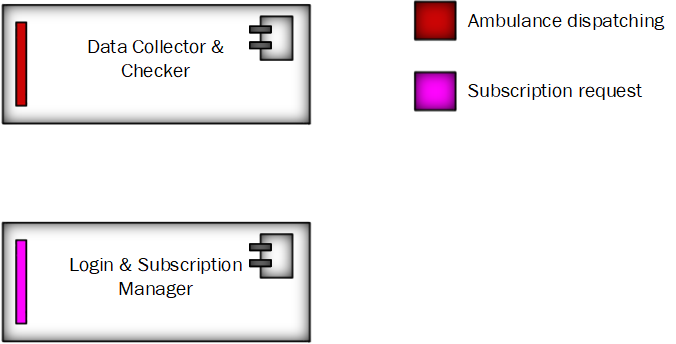
\includegraphics[scale=0.45]{pictures/ASOS_DependencyDiagram.png}}
        \caption{Dependencies among ASOS components}
        \label{fig:ASOS_DependencyDiagram}
    \end{figure}
    
    \begin{enumerate}
        \item \emph{Ambulance dispatching}
    \end{enumerate}
    It is of capital importance for this feature (red rectangle in the \textbf{figure} \ref{fig:ASOS_DependencyDiagram}) to be functioning correctly, hence it has to be thoroughly tested (both function-wise, checking if the ambulance is called \emph{if and only if} the health data received from D4H is over the critical threshold, and performance-wise, verifying that the ambulance is called within 5 seconds after receiving the critical measurement). The only component that deals with it is the Data Collector $\&$ Checker, which analyses incoming data and eventually communicates with the ambulance service. Until the next feature is not integrated, this one can be tested using health data that cover all possible situations (warning the ambulance service that it will receive some false alarms).
    
    \newpage
    \begin{enumerate} [resume]
        \item \emph{Subscription request}
    \end{enumerate}
    This feature (purple rectangle in the \textbf{figure \ref{fig:ASOS_DependencyDiagram}}) allows an Individual to subscribe to ASOS and it works just like a D4H subscription. It involves both the Login $\&$ Subscription Manager, that receives the log in request from the user and checks through D4H Communicator Manager Interface if he/she is registered to D4H as an Individual, and the Data Collector $\&$ Checker, that performs the actual subscription request through D4H Request Manager Interface. After having integrated this feature, the ASOS system can be tested as a whole using real data.

\subsection{Track4Run}
    There are five features that can be identified in T4R, highlighted in \textbf{figure \ref{fig:T4R_DependencyDiagram}} below.
    
    \begin{figure}[h]
        \centering
        \makebox[\textwidth][c]{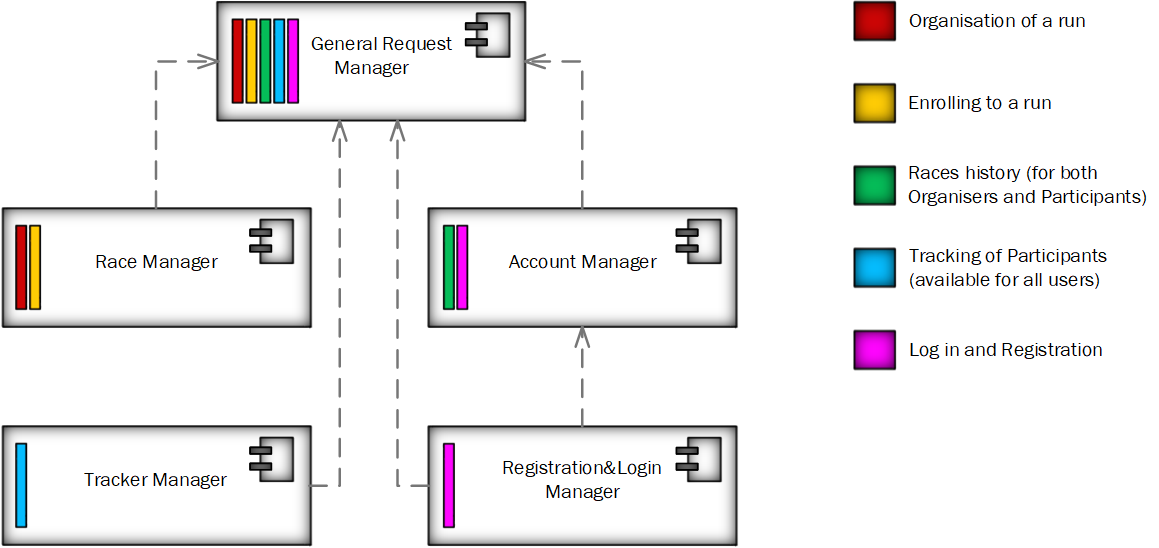
\includegraphics[scale=0.45]{pictures/T4R_DependencyDiagram.png}}
        \caption{Dependencies among T4R components}
        \label{fig:T4R_DependencyDiagram}
    \end{figure}

    The various functionalities will be implemented, integrated and tested in order of importance, with a thread for each feature. 
    
    \begin{enumerate}
        \item \emph{Organisation of a run}
    \end{enumerate}
    The first feature to implement and test is the possibility for Organisers to organise runs (red rectangle in \textbf{figure \ref{fig:T4R_DependencyDiagram}}), because the next ones can exploit it. This feature is encapsulated in the Race Manager component, aided by the General Request Manager to communicate with the Organiser Client.
    
    \begin{enumerate} [resume]
        \item \emph{Enrolling to a run}
    \end{enumerate}
    Having races available allows for Participants to enrol to them (yellow rectangle in \textbf{figure \ref{fig:T4R_DependencyDiagram}}), therefore this should be the next focus, so as to integrate the publish-enrol system and to test it as a whole. In this way, the development of the Race Manager will be completed and fully tested, along with another section of the General Request Manager.
    
    \newpage
    \begin{enumerate} [resume]
        \item \emph{Tracking of Participants}
    \end{enumerate}
    After the race management has been completed, the tracking system (light blue rectangle in \textbf{figure \ref{fig:T4R_DependencyDiagram}}) should be implemented and integrated, in order to test its functioning during a fully organised race. This feature is the only one that concerns the Tracker Manager, so this component will be fully integrated and tested by the time this thread reaches termination. Moreover, the part of the General Request Manager that forwards the tracking request consequent to an enrolment will be integrated.
    \\
    \begin{enumerate} [resume]
        \item \emph{Races history}
    \end{enumerate}
    At this point all the core functionalities of T4R have been integrated and tested, so the race history (green rectangle in \textbf{figure \ref{fig:T4R_DependencyDiagram}}), which is a support feature, should be developed and integrated next. The component responsible for this feature is the Account Manager, that communicates directly with T4R's database. It also exploits the General Request Manager in order to communicate with the Clients.
    
    \begin{enumerate} [resume]
        \item \emph{Log in and Registration}
    \end{enumerate}
    Finally, the log in and registration system (purple rectangle in \textbf{figure \ref{fig:T4R_DependencyDiagram}}) should be implemented, integrated and tested, so that Organisers can have their own account and Participants' previous registration to D4H can be checked. This last feature has its own dedicated component, aided by the General Request Manager for the communication with the Clients and by the Account Manager for the one with the database.
    
    
    
    
    
    
    
    
    
    
